\section{视网膜的输出}

\subsection{神经细胞感受野}
\begin{frame}
    \frametitle{神经节细胞的感受野}
    % \begin{columns}
        % \column{.5\textwidth}{
            中心-周边感受野的组织方式从双极细胞通过内网状层的突触传向神经节细胞。
            内网状层的无长突细胞的侧向链接也参与神经节细胞感受野的形成,但至今我们对这些连接的具体作用知之甚少。
        
            多数神经节细胞具有和上述双极细胞一样的同心圆式的中心-周边感受野结构。给光中心和撤光中心神经节细胞接收同类双极细胞的输入。
        
            多数视网膜神经节细胞对同时覆盖其感受野中心和周边的光刺激变化并无反应,主要对他们感受野内的\textbf{亮度差异}有反应。        
        % }\column{.5\textwidth}{
            \begin{figure}
                \centering
                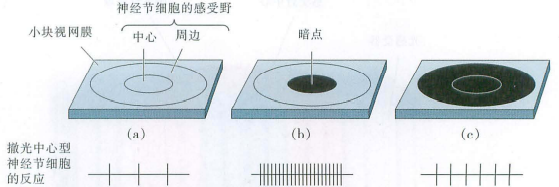
\includegraphics[width=.8\textwidth]{img/pic7-1.png}
                \caption{神经节细胞的中心-周边感受野\label{pic7-1}}
            \end{figure}
            \tiny{
                当一个暗点投射在撤光中心型神经节细胞的感受野中心时,细胞发放一串动作电位,但暗点范围扩大,则放电大幅减少。
            }
        % }
    % \end{columns}
    
\end{frame}

\begin{frame}
    \frametitle{神经节细胞感受野对明暗边界的调制}
    考察明暗边界对撤光中心神经节细胞输出的影响。根据实验,该信号有如图\ref{pic7-2}所示反应。%#TODO:做个图像分析
    \begin{figure}
        \centering
        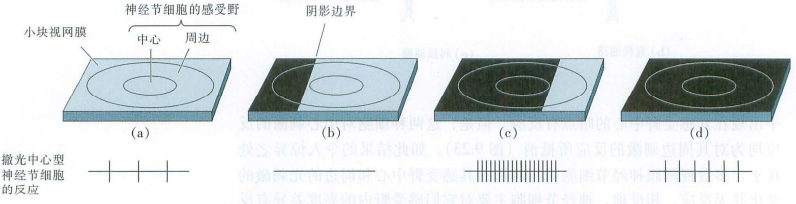
\includegraphics[width=.8\textwidth]{img/pic7-2.png}
        \caption{神经节细胞对感受野内明暗边界的反应\label{pic7-2}}
    \end{figure}
    从神经节细胞感受野的组织形式,我们可以推断,世界系统特化为对局部空间变化进行检测,而不是对于落在视网膜上光的绝对幅度进行检测,因此,\textbf{视网膜对光或暗的感知是相对的}。
\end{frame}
\subsection{神经细胞的类型}
\begin{frame}
    \frametitle{神经细胞按大小分类}

    在哺乳类视网膜,多数数神经节细胞具有一个中心-周边感受野,其中心区域或具给光反应或具撤光反应。他们可以进一步根据外形、突触连接、和
电生理特性进行分类。

在恒河猴和人体视网膜,已经发现两种主要 神经细胞:
    \scriptsize{
        \begin{itemize}
            \item 一种是大的\textbf{M型神经节细胞}(M-type ganglion cell),占神经节细胞总数的5\%;
            \item 另一种为小的\textbf{P型神经节细胞}(P-type ganglion cell),占神经节细胞总数的90\%;
            \item 其余的非M-非P细胞占5\%。
        \end{itemize}
    }

    M细胞具有较大的感受野,传导动作电位速度快,低对比度刺激更敏感。
    此外始于M细胞感受野中心的刺激为瞬时动作电位的发放,
    而对于P细胞则为和刺激时间等长的持续放电,如图\ref{pic7-3}。
    一种观点认为:M细胞对移动刺激的检测具有重要意义,而P细胞对刺激的形状及席位之处更敏感。
    \begin{figure}
        \centering
        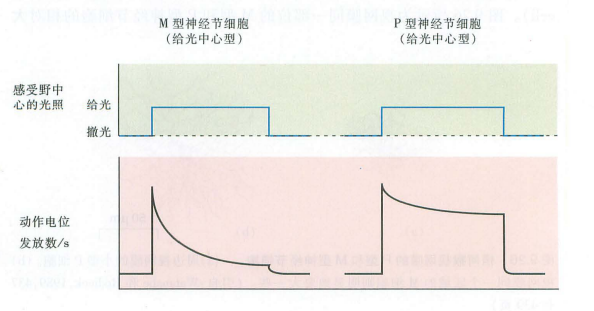
\includegraphics[height=.3\textheight]{img/pic7-3.png}
        \caption{M型和P型神经细胞的对光反应\label{pic7-3}}
    \end{figure}

\end{frame}
\begin{frame}
    \frametitle{神经细胞按颜色敏感性分类}

    视网膜神经节细胞间另一个差异在于P细胞和一些非M非P细胞对光的波长的敏感性差异。
    这些颜色敏感神经元的大部分称为\textbf{颜色对立细胞},
    反映了这种细胞的感受野中心对一种波长的反应可以为出现在感受野周边区域的另一种波长的光所抵消的事实。
    在P细胞,相互对立的颜色为蓝色和黄色。如图\ref{pic7-4},考虑红色给光中心和绿色撤光周边反应的细胞。
    %#TODO:没太看懂↑
    \begin{figure}
        \centering
        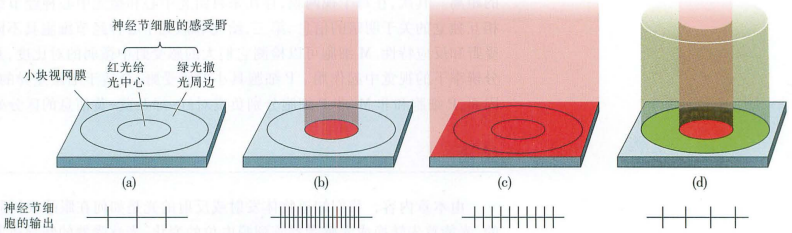
\includegraphics[width=.8\textwidth]{img/pic7-4.png}
        \caption{P型神经节细胞颜色对立的中心-周边感受野\label{pic7-4}}
    \end{figure}


\end{frame}

\subsection{并行处理}
\begin{frame}
    \frametitle{视觉系统的并行处理与信息整合需求概述}
    \begin{itemize}
        \item 由于我们是用两只眼睛看世界的,便产生了两个并行的信息流,在中枢系统中,这些信息流通过比较给出了关于深度(距离)的信息。
        \item 其次在每个视网膜,存在来自给光中心和撤光中心神经节细胞具有不同的感受野和反应特性,
        M细胞可以检测他们大的感受野中微弱的对比度,并在低分辨率下的视觉中起作用。
        P细胞据哟u小的感受野,合适于席位差异的检测。
        因此,P细胞和非M-非P细胞分别负责对红-绿及红-蓝信息的区分处理。
    \end{itemize}
    

\end{frame}